\documentclass[a4paper,12pt]{article}
\usepackage{fixltx2e}
\usepackage{amssymb}
\usepackage{hyperref}
\usepackage{pdfpages}
\usepackage{caption}
\usepackage{subcaption}
\begin{document}
\bibliographystyle{plain}
\title{Mesoscopic Modelling of Burst Suppression Under Anaesthesia}
\author{Matthew Walsh\\
   \small Brain and Psychological Sciences Research Centre (BPsyC),\\
   \small Swinburne University of Technology, Hawthorn, Victoria 3122, Australia; \\
   \texttt{matthew.walsh@gmail.com}\\
  \and
    David Liley\\
   \small  Brain and Psychological Sciences Research Centre (BPsyC),\\
   \small Swinburne University of Technology, Hawthorn, Victoria 3122, Australia; \\
   \small Cortical Dynamics Ltd, Hawthorn. Victoria 3122, Australia\\
   \texttt{dliley@swin.edu.au}}
\maketitle

\begin{abstract}
The burst suppression pattern is well recognized as
a major class of generalised electroencephlagram (EEG) waveform abnormality 
and is evoked by a variety of anesthetic agents. 
While the electroencephalographic phenomenon and clinical
implications of burst suppression have been studied extensively, the physiological mechanisms
underlying its emergence remain unresolved and obscure. 

While the model of Liley et. al. has been shown to account for many of the major features of the 
mammalian electroencephlagram, because of a strong coupling between excitatory and inhibitory population dynamics,  
it is unlikely to display burst suppression. This is because of the inability of simulated anesthetic action 
to induce the dynamics on multiple timescales that underlie bursting.
However the addition of a mean field driven slow wave system to the Liley model introduces 
multiple timescale behavior to the Liley model.

The extended Liley model is shown to exhibit burst suppression under physiologically 
plausible parameterisations for anesthesia with a wide variety of bursting behavior. 
This paper provides an overview of such dynamics and their relevance for a more 
complete physiological understanding of the EEG.

\end{abstract}
\section{Introduction}
Prior to the development of the modern intensive care unit in the early
1960s, featuring intubation, artificial respiration and comprehensive
physiological monitoring, reports of the electroencephalographic
pattern of burst suppression were confined to animal studies involving
deep anaesthesia and the odd case of psychosurgery~\cite{Niedermeyer2009}. Since then the burst suppression pattern is now well recognized as
a major class of generalised EEG waveform abnormality of diagnostic
and prognostic significance that is encountered in a range of
encephalopathic conditions, in addition to its pharmacological genesis
by a variety of sedative and anaesthetic agents. Typically the burst
suppression pattern consists of bursts of high amplitude slow, sharp or
spiking activity electroencephalographic activity separated by periods
of electroencephalographic suppression (isoelectricity). The oscillatory
features of the bursts, together with their duration and the duration of
suppressed periods show a high degree of variability (see Figure \ref{fig:burst_examples} for examples) that presumably reflects its
myriad of initiating causes. First identified
during deep anaesthesia with tribromoethanol in cats~\cite{Derbyshire31071936}, labelled “burst-suppression pattern” by Swank \& Watson~\cite{Swank01031949} during barbiturate and ether anaesthesia in dogs,
it is now
associated with cortical deafferentation~\cite{Henry19521},
cerebral anoxia and hypoxia, various types of intracortical lesions~\cite{FischerWilliams1963568}, deep coma, various infantile
encephalopathies, the final stages of deteriorated status epilepticus~\cite{Treiman199049}
, hypothermia, and high levels of many sedative
and anaesthetic agents~\cite{Schwartz1989}~\cite{Akrawi1996}

Burst suppression in the absence of anaesthesia is in general
associated with a very poor prognosis. Grigg-Damberger et al~\cite{GriggDamberger198984}
found that the neonatal appearance of burst suppression, even if
transient, was a portent of death or severe neurodevelopmental
disability in 93\% of infants who were followed up subsequent to the
appearance of electroencephalographic evidence of neonatal burst
suppression. In adult populations while an anoxic/hypoxic burst
suppression pattern signals a serious pathophysiological event the
outcome is not necessarily fatal and recovery with or without severe
neurological damage is possible~\cite{Niedermeyer2009}. The results of
experimental work with EEG monitoring in rats reveals that animals with
greater rates of high amplitude bursts had a better survival and
neurological outcome compared to those with lower rates of low
amplitude bursts~\cite{Geocadin2002193}.

While the electroencephalographic phenomenon and clinical
implications of burst suppression have been studied extensively~\cite{Niedermeyer2009}
(Brenner, 1985) the physiological mechanisms
underlying its emergence remain unresolved and obscure. However the
phenomenal resemblance of the patterns of burst suppression to
disorders of neuronal hyperexcitability suggests that similar
physiological mechanisms may be at root. For example the bursting
during burst suppression is often associated with myoclonic jerks
resembling those seen during epileptic fits. Further, during burst
suppression induced by various halogenated anaesthetic agents, bursts
can be readily evoked by auditory, visual or somatosensory stimuli
(Hartikainen et al, 1995). Like generalised epileptiform activity, bursts
are recorded simultaneously at multiple electrode derivations, implying
the wide synchronisation of neuronal activity. Not surprisingly then, in
clinical practice the boundaries between what constitutes coma
induced burst suppression and what is defined as ictal seizure activity
is blurred~\cite{Amzica2009} (Hirsch et al, 2004). While such
differentiation may be one of only semantics practically speaking there
nevertheless may be important clinical implications if they respond
differentially to pharmacotherapy and have different prognostic
outcomes, thus motivating attempts to better clarify such a
distinction.

Surprisingly many anaesthetic agents, at levels well below that needed
to induce burst suppression, quite commonly induce epileptiform
activity~\cite{Voss2008}. While such epileptiform activity rarely
progresses to clinically apparent seizures~\cite{GarciaMorales2009}
the presence of such activity nevertheless is believed to indicate some
form of incipient cortical hyperexcitability. Indeed a number of
mesoscopic mean field models developed to account for the
electroencephalographic features of anaesthetic action~\cite{Bojak2005}~\cite{SteynRoss1999}, based on parameterising empirically
identified sub-cellular and molecular targets, have been able to account
for the pro-convulsant properties of many anaesthetic agents known
to have seizurogenic potentia~\cite{Liley2005}l (Wilson et al, 2006;). Given that the majority of anaesthetic agents induce burst
suppression it is therefore natural to inquire whether these mesoscopic
mean field models of electrocortical anaesthetic action are able to
account for the appearance of drug-induced burst suppression, and in
doing so shed light on the pathophysiological mechanisms of burst
suppression and epilepsy in general.

\begin{figure}
	\label{fig:burst_examples}
	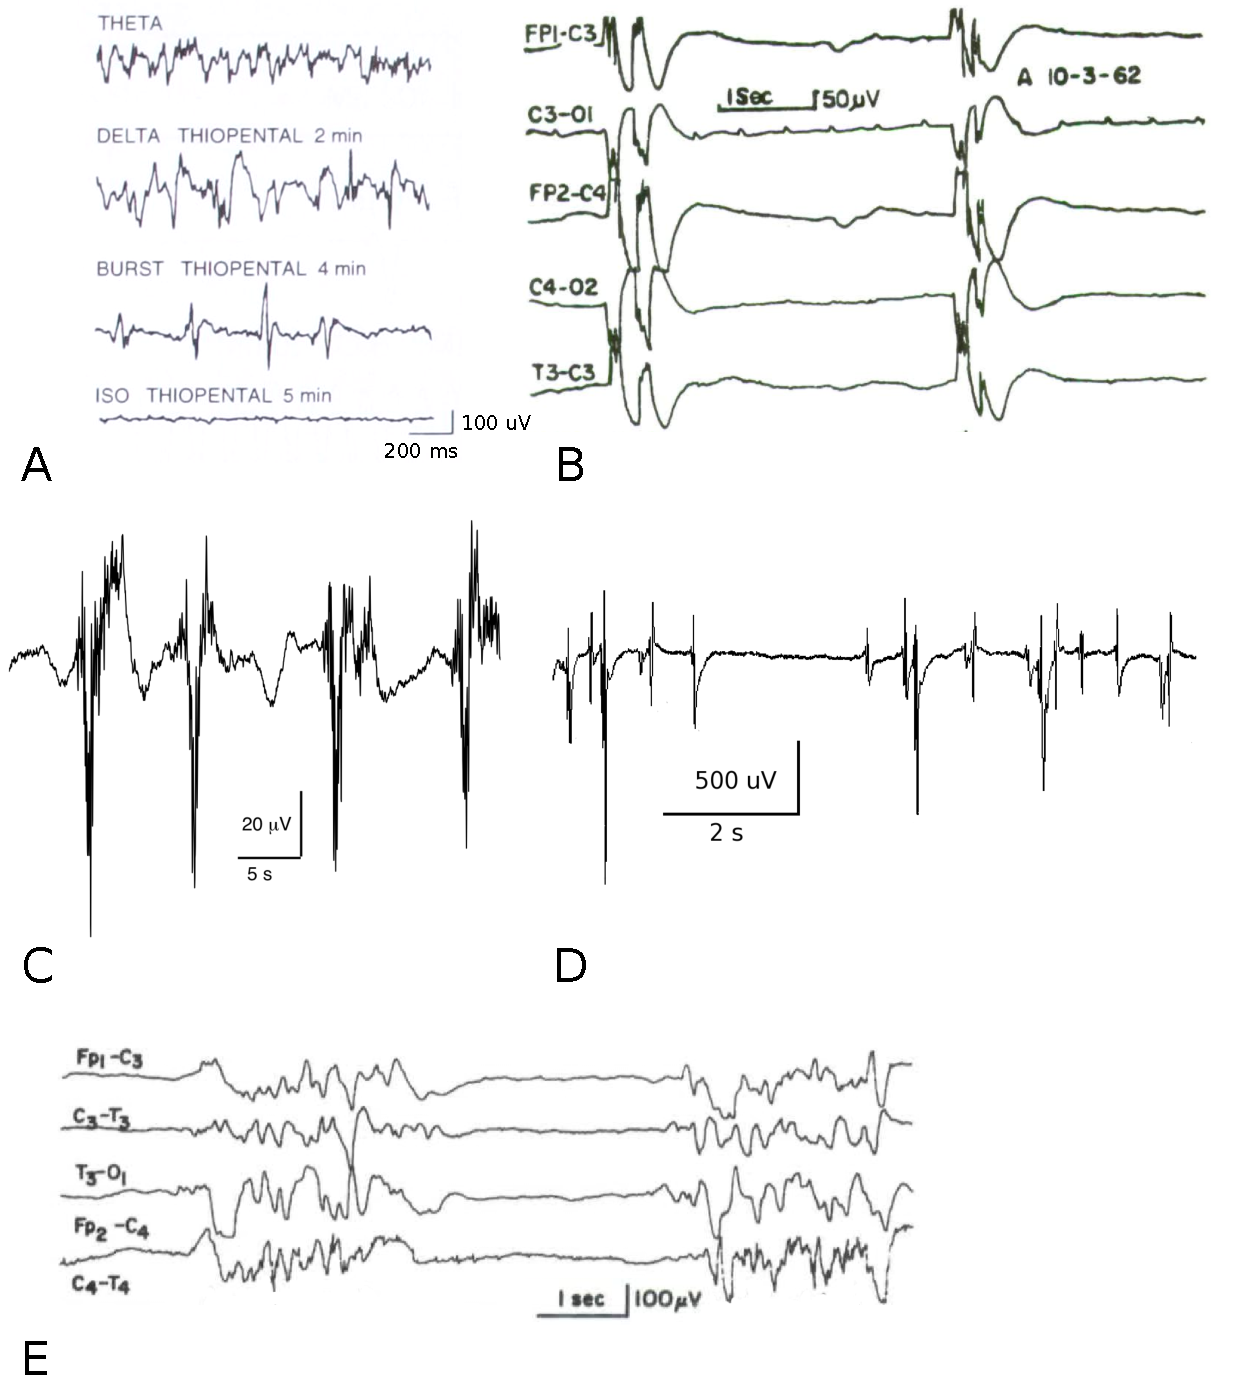
\includegraphics[scale=0.7]{chosen-frontiers-2012/burst_examples.pdf}
	\caption{Example traces of electroencephalogram and
electrocorticogram illustrating the heterogeneity of burst suppression
patterns. (A) changes in neocortical electroencephalogram in the rat,
recorded using dural surface electrodes, in response to a 5 mg/kg/min
thiopental infusion (figure reproduced with permission from Lukatch \&
MacIver, 1996). (B) electroencephalogram recorded in acute anoxia
showing a clear burst suppression pattern with grouped spikes (figure
reproduced with permission from Hockaday et al, 1965). (C) burst
suppression pattern during closed loop target controlled propofol
infusion at a target level of approximately 15 μg/ml (data courtesy of
Professor Michel Struys, Groningen). Note the bursts consist of fast
activity ($>$ 10 Hz) on a slow wave background. (D) electrocorticogram
obtained from an adult merino sheep during deep enflurane anaethesia,
demonstrating high amplitude spikes interspersed with isoelectric
periods of variable length (figure reproduced with permission from
Voss et al, 2006). (E) electroencephalogram recorded from a 3 month
old infant suffering from infantile myoclonic encephalopathy
(reproduced with permission from Niedermeyer, 2005).}
\end{figure}

\section{Methods}
\subsection{Mesoscopic mean field modelling of electrocortical activity}
The electroencephalogram and electrocorticogram arise out of the
cooperative activity of many thousands of neurons. A single
electroencephalographic electrode records the synaptically induced
currents of well over a 100,000 neurons (Nunez \& Srinivasan, 2006)
and thus detailing each neurons contribution to this summed activity
would appear superfluous. For this reason it is preferable instead to
model the activity of populations of neurons. One general way of
achieving this, in which known stochastic fluctuations can be included,
is to dynamically evolve the probability distributions associated with
the states of the neuronal ensemble. While in principle providing a
rigorous way forward the formulation of such stochastic equations of
motion entails a great deal of physiological uncertainty. For this and
other reasons (Deco et al, 2008) a more resolute path is to
dynamically evolve some average quantity such as the mean soma
membrane potential or the mean firing rate of some suitably defined
neuronal ensemble. In this manner a mesoscopic level model can be
developed which acts as a bridge between cellular (or microscopic)
level activity and whole brain (or macroscopic) level behaviour.
While the current mathematical approach for formulating the equations
of motion for the activity of neuronal populations or masses, stems
principally from the works of Wilson \& Cowan (1973, 1972), Nunez
(1974), Freeman (1975) and Amari (1975, 1977), they are not
particularly successful in articulating the genesis of rhythmic activity in
the EEG and its modulation by pharmacological agents, due to a range
of mathematical simplifications that cannot be justified by an appeal to
physiology. For this reason a range of biologically more refined
neuronal populations models have been developed (Deco et al, 2008)
that form a more appropriate basis from which to model the
physiological genesis of the electroencephalogram. The model of Liley
et al (2005; 2003; 2002; 1999) is one such model and will be the
focus of our attempts to account for the phenomenon of burst
suppression.

The model of Liley et al (2011; 2005; 2003; 2002; 1999) is able to
account for the major features of the mammalian
electroencephalogram in the context of a parameterisation that
accords with physiological measurement and experiment. Because it
aims to provide a dynamical description of the electroencephalogram
the model is spatially coarse-grained over the approximate extent of a
cortical macrocolumn, reflecting the general physiological wisdom that
such columniation signifies populations of neurons having similar
functional behaviour and anatomical connectivity. The multiple
interactions between individual neurons are replaced by effective feed-forward
and feed-back interactions between the mean activity (or
“mean fields”) of excitatory and inhibitory populations of neurons over
the spatial extent of the column. In this way mammalian neocortex is
conceived as consisting of localized populations of excitatory and
inhibitory neurons interacting by all possible combinations of
feedforward and feedback connectivity interacting globally via long
range excitatory connections (Figure \ref{fig:liley_schema}).

\begin{figure}
\label{fig:liley_schema}
		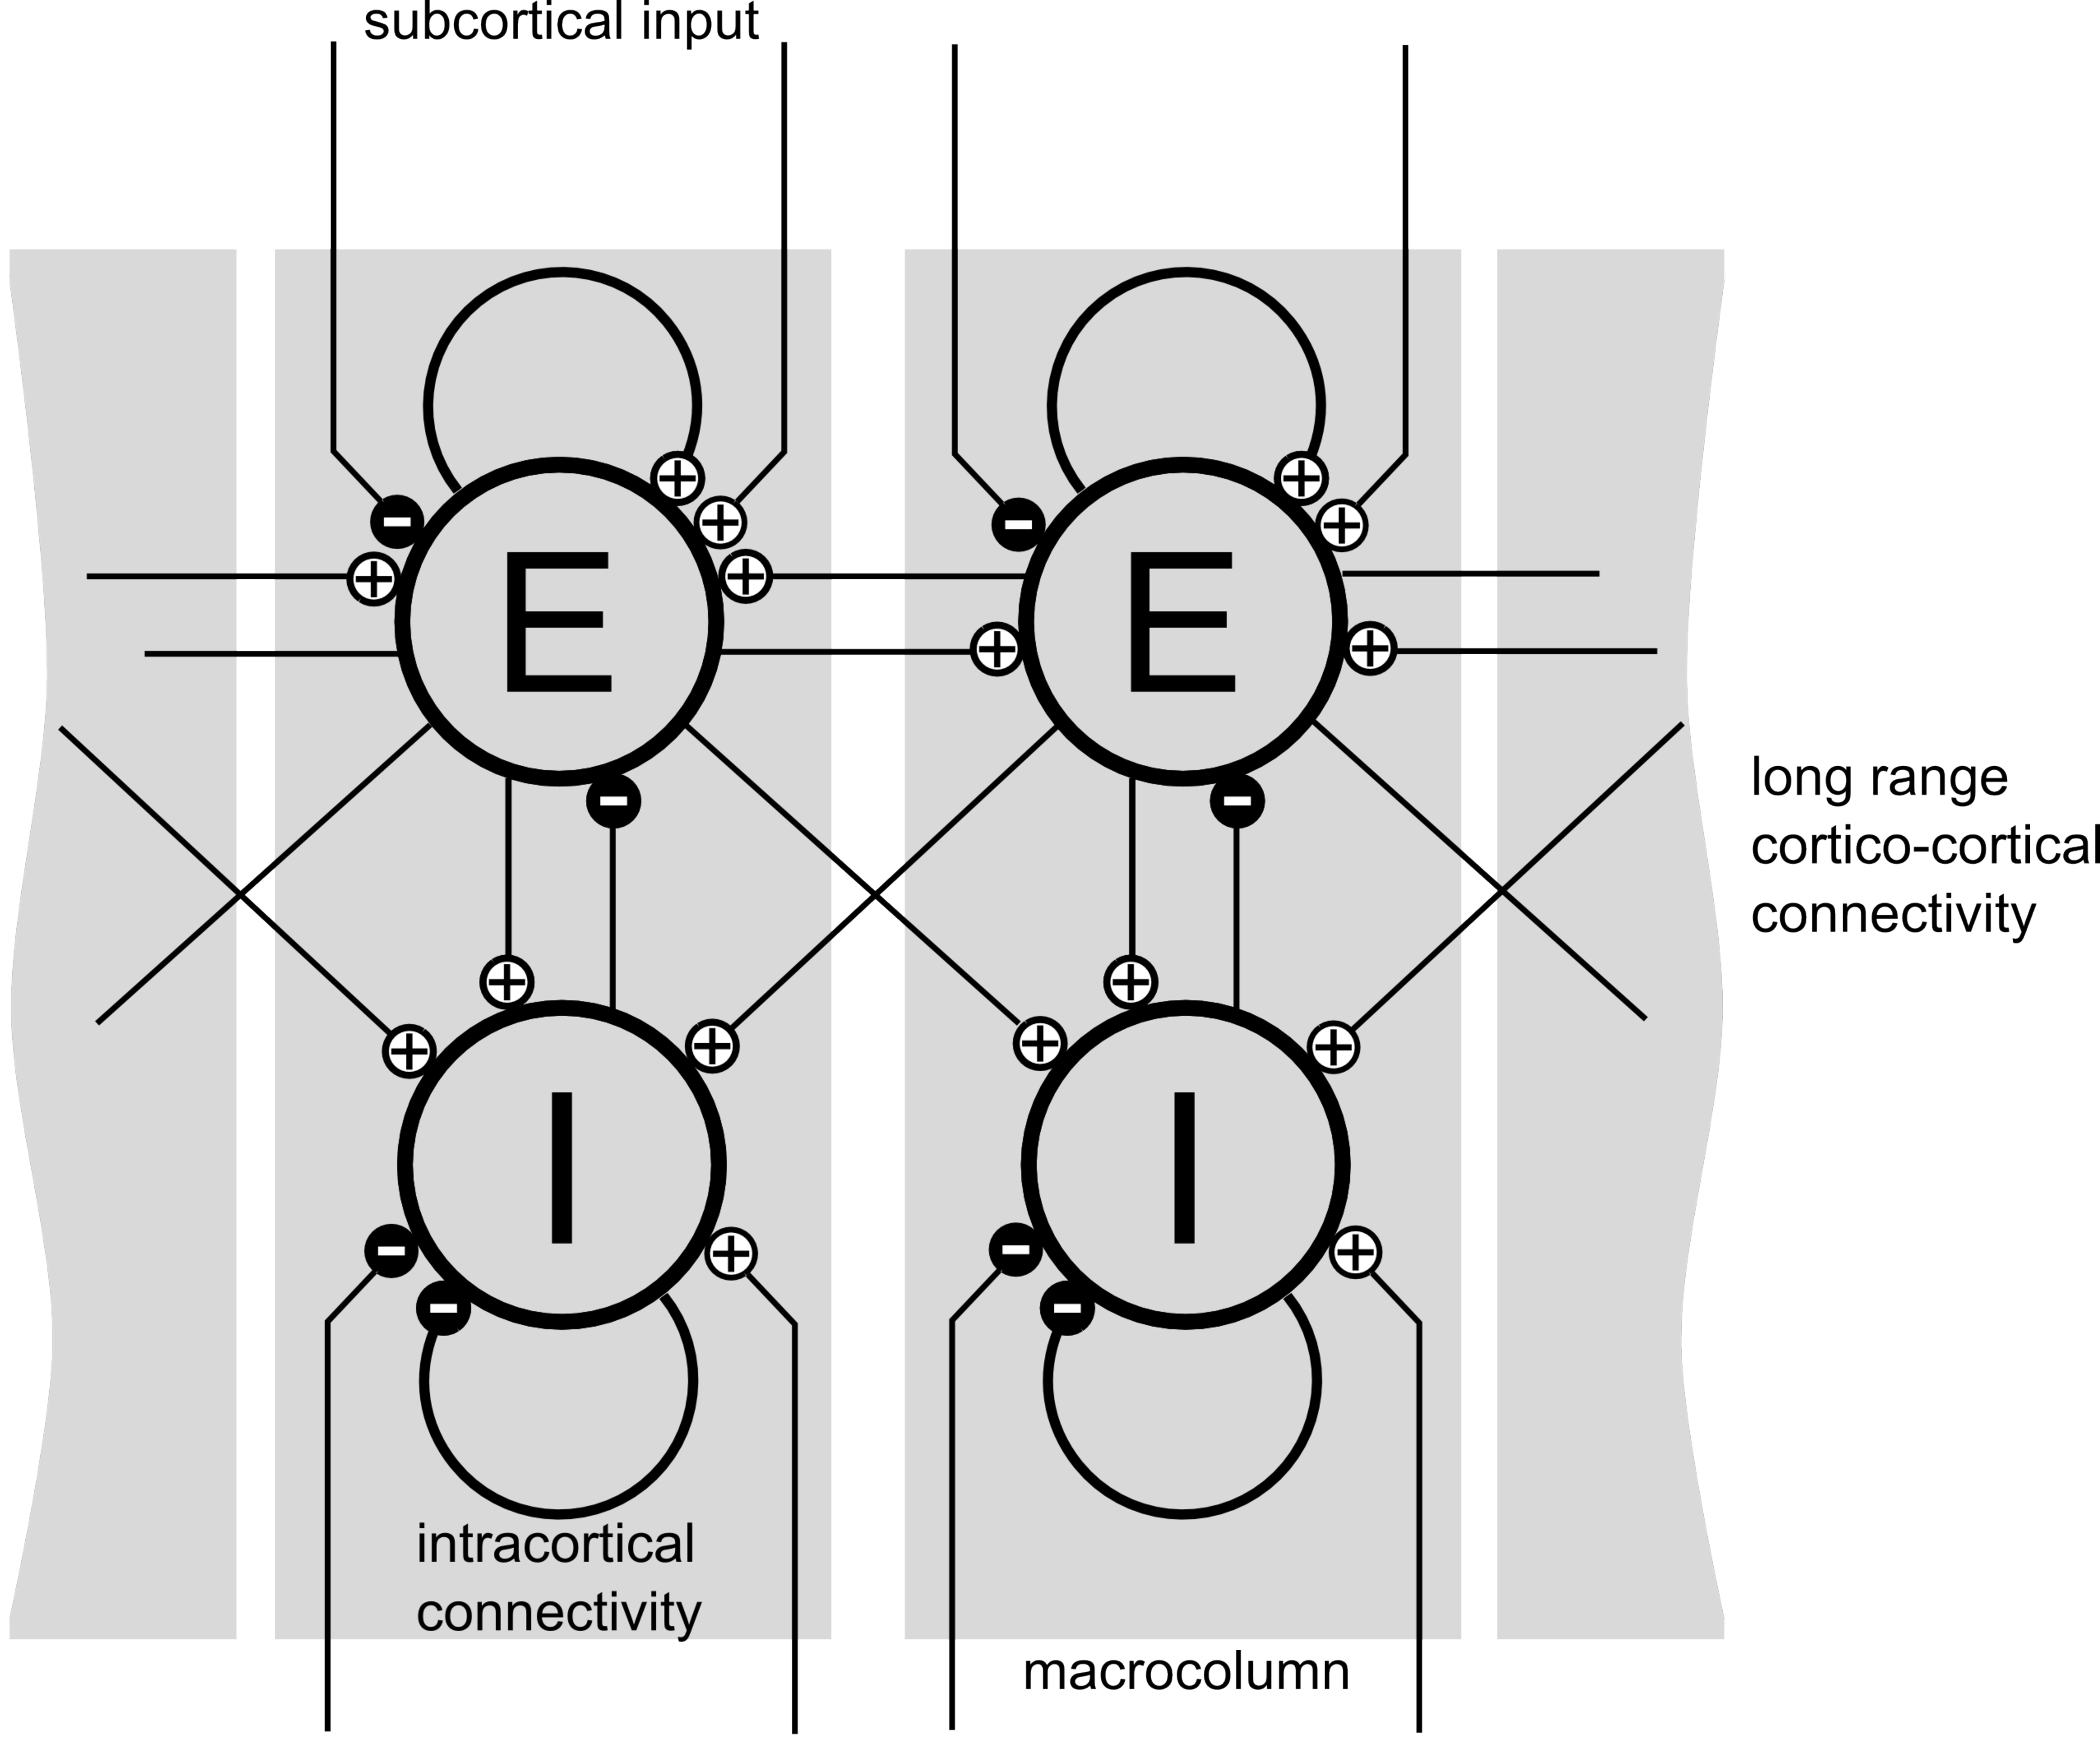
\includegraphics[scale=0.15]{chosen-frontiers-2012/liley_topology.pdf}
		\caption{Schematic overview of the essential intracortical and corticocortical
interactions between excitatory and inhibitory neuronal
populations in the model of Liley et al (2011; 2005; 2003; 2002;
1999). Figure reproduced with permission from Liley et al (2011).
Following conductance based approaches typically used to model
networks of synaptically interacting networks of individual model
neurons, excitatory and inhibitory neuronal populations are modeled as
single passive resistive-capacitive compartments into which all
synaptically induced postsynaptic currents flow. Functionally these
populations are equivalent to the excitatory and inhibitory KO sets of
Freeman’s (1975) K-set hierarchy. Cortical activity is then described
by the mean soma membrane potentials of the spatially distributed excitatory ($h_e$)
and inhibitory ($h_i$) neuronal populations. The connection with physiological measurement is obtained through $h_e$,
which is
assumed to be linearly related to the surface recorded
electroencephalogram (Nunez \& Srinivasan, 2006; Freeman, 1975).}
\end{figure}

Thus the response of the mean soma membrane potential $h_k$ ($k=e,i$) at position $r$ on a two dimensional cortical
sheet, to induce post synaptic activity $I_{lk}$ ($l$=source, $k$=target population) is given by

\begin{equation} \label{eq:h_k} 
\tau_k\frac{\partial h_k(r,t)}{\partial t} = h^r_k - h_k(r,t) + \sum_{l=e,i} \frac{h_{lk}^{eq} - h_k(r, t)}{\left|
h_{lk}^{eq}-h_k^r\right|}I_{lk}(r,t)
\end{equation}

The postsynaptic response to a single pre-synaptic action potential (at
t = 0) is modeled by the well-known synaptic alpha function of cable
theory as $\Gamma_{lk} \gamma_{lk}t\exp(1-\gamma_{lk}t), t \geq 0$ and is excitatory or inhibitory depending
on the sign of $\Gamma_{lk}$ (peak amplitude), and thus we assume that the time
course of the synaptically induced excitatory and inhibitory currents is
described by a critically damped oscillator driven respectively by the
mean rate of incoming excitatory and inhibitory axonal pulses:

\begin{equation} \label{eq:i_lk}
\left( \frac{\partial}{\partial t} + \gamma_{lk} \right)^2 I_{lk}(r,t) = \exp(1)\Gamma_{lk}\gamma_{lk}.A_{lk}(r,t)
\end{equation}
\noindent
With
\begin{equation} \label{eq:a_ek}
A_{ek}(r,t) = N_{ek}^{\beta} S_e[ h_e(r,t)] + \phi_{ek} + p_{ek}(r,t)
\end{equation}
\noindent
And
\begin{equation} \label{eq:a_ik}
A_{ik}(r,t) = N_{ik}^{\beta} S_i[h_i(r,t)] + p_{ik}(r,t)
\end{equation}
\noindent
where $A_{lk}$ comprises the different sources of presynaptic spikes: $N_{lk}^\beta S_i$ (input from local cortical
neuronal populations), $\phi_{ek}$ (input from long range excitatory cortico-cortical fibres) and $p_{lk}$
(extracortical sources).
While the present consensus is that extracortical sources
(thalamocortical afferents) are purely excitatory in nature and thus $p_{ik} \cong 0$, we choose to keep these terms as
they enable the effects of
tonic inhibition to be included without the need to define additional
parameters. The time courses of the synaptically induced currents, $1 / \gamma_{lk}$ are taken to describe the time
course of ‘fast’ excitatory ($l = e$: $\alpha$-amino-3-hydroxl-5-methyl-4-isoxazole-propionate (AMPA) \& kainate) and
inhibitory ($l=i$: $\gamma$-amino-butyric-acid type A (GABA\textsubscript{A}) neurotransmitter kinetics. Mean neuronal
population firing rates, $S_l$, are assumed to to instantanious sigmoid functions of the mean soma membrane potential
i.e

\begin{equation} \label{eq:s_l}
S_l[h_l(r,t)]=S_l^{max}/\{1 + \exp[\sqrt{2}(h_l(r,t)-\mu_l)/\sigma_l]\}
\end{equation}

The axonal pulses $\phi_{ek}$ propagated by the exclusively excitatory long
range cortico-cortical fibre system is in the simplest case described by
the following two-dimensional telegraph equation,

\begin{equation} \label{eq:phi}
\left(\frac{\partial}{\partial t} + v_{ek} \Lambda_{ek} \right)^2 \phi(r,t) - \frac{3}{2} v_{ek}^2
\nabla^2\phi(r,t)=v_{ek}^2 \Lambda_{ek}^2 N_{ek}^\alpha S_e[h_e(r,t)]
\end{equation}

where $N_{ek}^\alpha$ is the total number of excitatory connections formed by
long range cortico-cortical axons on long on local population $k$, and
assumes a single axonal conduction velocity $v_{ek}$ and and an exponential fall
off with distance (characteristic scale = $1/\Lambda_{ek}$) of the strength of
cortico-cortical connectivity. For simplicity, and given the fact that in
anaesthesia burst suppression involves the whole brain, we chose to
only study the spatially homogeneous case i.e. $\nabla^2 = 0$

Equations (\ref{eq:h_k}, \ref{eq:i_lk}, \ref{eq:a_ek}, \ref{eq:a_ik} \& \ref{eq:phi}) represent a system of 8 coupled
non-linear partial
differential equations that typically defines the Liley model of
electrocortical rhythmogenesis, which is capable of reproducing the
main features of spontaneous human electroencephalogram (alpha
resonance, $'1/f'$ activity). Table \ref{table:model_params} summarises all model parameters,
their definitions and approximate ranges. 

\begin{table}[h]
\label{table:model_params} 
\begin{tabular}{r l r r l}
\hline 
 & Definition & Min & Max & Units \\
\hline
$h_k^r$ & resting membrane potential & −80 & −60 & $mV$ \\
$\tau_k$ & passive membrane decay time & 5 & 150 & $ms$ \\
$h_{ek}^{eq}$ & excitatory reversal potential & −20 & 10 & $mV$ \\
$h_{ik}^{eq}$ & inhibitory reversal potential & −90 & $h_k^r - 5$ & $mV$ \\
$\Gamma_{ek}$ & EPSP peak amplitude & 0.1 & 2.0 & $mV$ \\
$\Gamma_{ik}$ & IPSP peak amplitude & 0.1 & 2.0 & $mV$ \\
$1/\gamma_{ek}$ & EPSP rise time to peak & 1 & 10 & $ms$ \\
$1/\gamma_{ik}$ & IPSP rise time to peak & 2 & 100 & $ms$ \\
$N_{ek}^\alpha$ & number of excitatory cortico-cortical synapses & 1000 & 5000 & − \\
$N_{ek}^\beta$ & number of excitatory intracortical synapses & 2000 & 5000 & − \\
$N_{ik}^\beta$ & number of inhibitory intracortical synapses & 100 & 1000 & − \\
$v_{ek}$ & axonal conduction velocity & 0.1 & 1 & $mm/ms$ \\
$1 / \Lambda_{ek}$ & decay scale cortico-cortical connectivity & 10 & 100 & $mm$ \\
$S_k^{max}$ & maximum firing rate & 0.05 & 0.5 & $ms^{-1}$ \\
$\mu_k$ & mean firing threshold & −55 & −40 & $mV$ \\ 
$\sigma_k^2$ & variance in firing threshold & 4 & 49 & $mV^2$ \\
$p_{lk}$ & extracortical synaptic input rate & 0 & 10 & $ms^{-1}$ \\
\hline
\end{tabular}
\caption{List of spatially averaged parameters for different types $k,l \in \{e,
i\}$ of neuronal target populations in the electrocortical model of Liley et
al. (2011; 2005; 2003; 2002; 1999), with typical ranges that are
assumed to be physiologically admissible. Table adapted from Liley et
al (2011).}
\end{table}

\subsection{Model parameterisation: generation of normative parameter sets}
Because burst suppression activity (at least that caused by
anaesthetic and sedative action) is assumed to ultimately arise out of
a background of normal electroencephalographic activity it is
important to define parametrically normative states in order to study
how they may be perturbed during health and disease. We therefore
chose to utilize previously defined parameter sets (Bojak \& Liley,
2005) that have the following properties: i) are confined to the
physiologically admissible parameter space (see Table 1), ii) give rise
to electroencephalographically and physiologically plausible activity
($'1/f'$ decay at low frequencies plus a relatively sharp peak at alpha
frequencies, 8 – 13 Hz; mean excitatory/inhibitory neuronal firing rates
$< 20 s^{-1}$) and iii) that exhibit transient increases in total power and
monotonic reductions in mean frequency with respect to modeled
anaesthetic action (see below). In general such sets are found by
randomly searching the high dimensional physiologically admissible
(and plausible) parameter space. For further details see Bojak \& Liley
(2005).

\begin{table}[h]
\label{table:site_of_action} 
\begin{tabular}{p{5cm} p{5cm} l}
\hline 
 Site of action & Main anaesthetic effect & Parameters \\
\hline
2PK channels \& extrasynaptic GABA$_A$ receptors & increase in tonic inhibition & $p_{ik}, h_k^r$ \\
\\
HCN1 pacemaker channels & membrane hyperpolarisation, increase in EPSP amplitude$^a$ & $\Gamma_{ee}, h_e^r$\\
\\
nACh receptors & reduction in tonic excitation & $p_{ek}, h_k^r$ \\
\\
synaptic GABA$_A$ & increase in IPSP charge transfer & $\Gamma_{ik}, \gamma_{ik}$\\
\\
AMPA/kainate \& NMDA$_b$ receptors & decrease in EPSP charge transfer & $\Gamma_{ek}, \gamma_{ek}$\\
\\
myelinated axons$^c$ & decreased conduction velocity & $v_{ek}$\\
\\
Na channels & alterations of neuronal firing & $S_k^{max}, \mu_k, \phi_k$\\
\hline
\end{tabular}
\caption{Relationship between major experimentally identified sites of
cortical anaesthetic action and parameters of the electrocortical model
of Liley et al. (2005; 2003; 2002; 1999). EPSP = excitatory
postsynaptic potential; IPSP = inhibitory postsynaptic potential; 2PK =
two-pore potassium; nACh = nicotinic acetylcholinergic; NMDA = Nmethyl-
d-aspartate; $^a$ only demonstrated in excitatory neurons (Chen
et al, 2009). $^b$ hypothesized to depend on $h_k$ ; $^c$ Effect demonstrated
in periphery, speculative in cortex (Swindale, 2003). Table adapted
from Liley et al (2011).}
\end{table}



\subsection{Investigating and incorporating speculative physiological
mechanisms of burst suppression}
While it is often assumed that burst-suppression pattern arises from
slow thalamic oscillations driving cortex (Fisch, 1999), the fact that
this pattern persists subsequent to cortical deafferentation instead
suggests that it is an intrinsic dynamical feature of cortical tissue
(Luktach et al, 1995).
While many anaesthetic agents, at sufficiently high doses, are capable
of producing burst suppression pattern electroencephalogram, not all
do. Pharmacologically, anaesthetics that induce burst suppression all
seem to have a GABAergic profile, even if weak. One that has not
been reported to induce burst suppression, xenon, is widely believed to
act principally via the antagonism of glutamatergic neurotransmission.
Indeed it is reported in laboratory slice preparations that burst
suppression induced by thiopental, propofol and isoflurane requires the
maintenance of glutamate-mediated excitatory neurotransmission
(Luktach et al, 2005). While NMDA antagonists have been shown to
reduce burst duration and amplitude in slice preparations (Kroeger \&
Amzica, 2007), in clinical practise antiepileptic drugs generally show
poor response.
Lukatch \& MacIver (1996) report that burst suppression appears to
result from the direct activation of GABA-gated Cl– channels as
muscimol, a potent selective GABAA agonist, reliably induces this
phenomenon. Therefore perturbation of GABAergic neurotransmission
may be key to understanding the pathophysiology of burst
suppression. Such a view is also supported by work involving
hippocampal slices subject to simulated ischemia in which it is found
that ischemia releases GABA initially by exocytosis and then by
reversal of a high affinity GABA plasma membrane transporter (GAT-1;
Allen et al, 2004).
The implied importance of GABAergic inhibitory processes is also
supported by the work of Steriade et al (1994) in which they found
that hyperpolarisation of the resting cell membrane potential of
cortical neurons reliably preceded conspicuous electroencephalographic
aspects of burst suppression. However in addition to inhibitory
GABAergic contributions they also ascribed the hyperpolarisation to i)
thalamic disfacilitation ii) inactivation of a variety of inward ionic
currents and iii) increases in membrane K+ conductances.
While maintenance of a sufficient level of glutamate-mediated
excitatory neurotransmission is required for the genesis of the bursting
in burst suppression, there is nevertheless evidence that
neurotransmission in general is attenuated. For example Kroeger \&
Amzica (2007) showed that bursting depleted interstitial Ca2+ to a
level incompatible with synaptic transmission, and speculate that this
accounts for the isoelectric suppression period. That attenuated
neurotransmission may also be involved in the genesis of hypoxia
induced burst suppression is supported by the works of Endemli and
Crunelli (1998), in which they found that brief periods of anoxia can
cause a total, but reversible loss of synaptic transmission, and
Fleidervish et al (2001), in which it was found that hypoxia depleted
readily releasable pools of vesicles for transmitter release.

\subsection{Theoretical basis of busrting}
Bursting in single neuron models has been acheived by modelling neuronal behaviour on multiple timescales~\cite{izikevich2007_1}. 'Fast' timescale(s) ($\tau^{fast}$) must be present, underlying a fast system that drives the active spiking phases of bursting. 'Slow' timescale(s) ($\tau^{slow}$) must also be present, underlying the quiescent periods of suppression. The fast and slow timescales must significantly differ, with $\tau^{fast} \ll \tau^{slow}$. 

The mean field model of Liley et al was inspected in an attempt to identify differing timescales that could bring about BS in a similar fashion to the bursting induced in single neuron models. 

Liley et al (Liley et al, 2003 - Drug-induced modification of the system properties associated
with spontaneous human electroencephalographic activity) propose that oscillatory activity within cortical interneuron
(inhibitory) circuits is generated by a feedback mechanism between the excitatory and inhibitory population.
The inhibitory population activity phase leads excitatory population activity, generating a phase locked system of
inhibitory and excitatory neurons generating the observed oscillatory behaviour. The phase locking of these systems leads us to assume that equations \ref{eq:h_k} and \ref{eq:i_lk} represent a single 'fast'
timescale within the model of Liley et al. 

No obvious candidate for a slow timescale in the cannonical model of Liley et al existed, thus additional physiologically plausible slow systems were introduced as augmentations to the cannonical mean field model of Liley et al. The long range coupling described in \ref{eq:phi} was also identified as a possible candidate for an emergent slow timescale via parametric alteration.

\subsection{Introduction of a simple 'thalamus'}

Cortico-Thalamic feedback has been proposed as a mechanism for the generation of slow sleep waves (ref steriade etc) and its plausibility as a slow timescale system leading to BS in the mean field model of Liley et al was investigated. Thalamic feedback was modelled as a simple, first order, low pass filtering of mean field activity. This was acheived by introducing a mean field  thalamic averaging (TA) model $\zeta$. As cortico-thalamic connections are almost entirely excitatory in nature(ref) it was assumed $\zeta$ was driven proportionally to the firing rate of the excitatory system $S_e(h_e)$.
A simple first order low pass filter was used for $\zeta$, represented by the following coupled ordinary differential equation

\begin{equation} \label{eq:zeta_slow} 
\tau^{slow} \frac{\partial \zeta}{\partial t} = g S_e(h_e) - \zeta
\end{equation}
where $\tau^{slow}$ is the time constant for the filter and $g$ is a dimensionless constant for mean field connectivity.

The extra cortical input $p_{ek}$ in (\ref{eq:a_ek}) was reformulated to include a component of cortico-thalamic feedback. This feedback component was assumed to be linearly proportianal to $\zeta_e$. Thus the constants for $p_{ek}$ in (\ref{eq:a_ek}) were replaced with the expression

\begin{equation} \label{eq:p_ek}
p_{ek} = \hat{p}_{ek} + \rho_{ek} \zeta
\end{equation}
\noindent
Where $\rho_{ek}$ is a dimensionless constant of connectivity to $\zeta$. $\hat{p}_{ek}$ is a constant that represents
the purely feed-forward component of extra cortical input and corresponds with the original constant expression for $p_{ek}$ in the cannonical model. 

It should be noted that when $\rho\zeta=0; \forall t \geq 0$ this augmented model collapses back to the cannonical model of Liley et al.

\subsection{Intracellular and/or synaptic resource utilisation}
(Tsodyks and Markram 1997, Bazhenov et Al 2002) introduced generic neuronal models of synaptic resource utilisation and recovery. Spiking activity expends neuronal resources and bursting can come about through inadequate recovery thus leaving the neurons in a depleted state.  Similarly a model of intracellular and synaptic resource utilisation (SIRU) was introduced in to the mean field model of Liley et al. 

In the mean field model of Liley et al, it was assumed that a depletion in intracellular or synaptic resources would present itself as a decrease in the peak PSP. Therefore we reformulated the peak excitatory PSPs ($\Gamma_{ek}$, where $k \in \{e, i\}$) to
introduce a simple model of synaptic/intracellular resource utilisation.

The rate of change of the peak excitatory PSP can be expressed as a simple logistic equation where:
\begin{equation}
\label{eq:res_rate}
\frac{\partial{\Gamma_{ek}}}{\partial{t}} = R_{ek}^{recovery} - R_{ek}^{depletion}
\end{equation}
\noindent
Where $R_{ek}^{recovery}$ is the rate of peak PSP recovery and $R_{ek}^{depletion}$ is the rate of peak PSP depletion.

$R_{ek}^{recovery}$ is assumed to be proportional to the decrease in peak PSP ($\hat{\Gamma}_{ek} - {\Gamma}_{ek}$), giving
\begin{equation}
\label{eq:res_recov}
R_{ek}^{recovery}= \frac{\hat{\Gamma}_{ek} - {\Gamma}_{ek}}{\tau_{ek}^{slow}}
\end{equation}
\noindent
Where $\tau_{ek}^{slow}$ is the time constant for peak PSP recovery, $\hat{\Gamma}_{ek}$ is the original constant expression for $\Gamma_{ek}$ that represents the nominal peak PSP.

$R_{ek}^{depletion}$ is assumed to be proportional to the excitatory firing rate $S_e(h_e)$ and the current peak PSP ($\Gamma_{ek}$), giving
\begin{equation}
\label{eq:res_depl}
R_{ek}^{depletion}= \frac{\Gamma_{ek} \chi_{ek}S_e(h_e)}{\tau_{ek}^{slow}}
\end{equation}
\noindent
Where $\chi_{ek}/\tau_{ek}^{slow}$ is the resource depletion time constant.

Substituting (\ref{eq:res_recov}) and (\ref{eq:res_depl}) into (\ref{eq:res_rate}) gives
\begin{equation} \label{eq:Gamma_ek}
{\tau^{slow}_{ek}} \frac{\partial{\Gamma_{ek}}}{\partial{t}} = \hat{\Gamma}_{ek} - \Gamma_{ek}(1 + \chi_{ek} S_e(h_e))
\end{equation}

It should be noted that when $\chi_{ek}=0$ and $t \gg 0$ this model aproaches the cannonical model of Liley et al.

\subsection{Emergence of a slow timescale from a parametric variation in the cannonical model}
While the coupled inhibitory/excitatory system represents a single fast timescale in the mean field model of Liley et al, there is also a long range coupling system ($\phi_{ek}$). This system describes long range intra-cortical connections. The possibility that this system could operate on a slower timescale through parametric variation and thus inducing BS was investigated.

Swindale 2003 hypothesises that anaesthesia may bring about changes to axonal conduction velocities and capacitances. Furthermore it is known that hypothermia significantly affects conduction velocities(ref) and is also a known condition under which BS occurs. We investigated the
effects of modifying the conduction velocity and the characteristic decay scale ($v$ and $\Lambda_{ek}$) had on the
long range coupling $\phi_{ek}$ system, in an attempt to bring about slow oscillations in this system.

\subsection{Simulation of anaesthetic induction}
Anaesthetic induction can be simulated within the mean field model of Liley et al via parametric alterations. Present knowledge of parameters that are modified due to anaesthetic action is restricted to parameters within the cannonical model (see Table \ref{table:model_params}). The contribution that known anaesthetic effects have on the instigation of BS and its dynamics were studied by simulating anaesthetic induction in the presence of slow timescale systems. 

The simulation of anaesthetic induction concentrated on varying the model parameters $\Gamma_{ik}$ and $\gamma_{ik}$ as these parameters are known to vary with GABAergic anaesthetics. 

\subsection{Computational methods}
Riznel (1995) introduces a method of dissection to analyse systems that operate on multiple timescales. Fast and slow systems are considered separately and the slow system can be frozen, replacing it with a parameter in the fast system. This frozen system can then be used to analyse the dynamics of the fast system with respect to the slow system. Izhikevich (ref) introduces common bursting topologies, where the transitions between quiescence and spiking can be viewed as bifurcations with respect to the frozen slow parameter(s).

A large scale numerical bifurcation analysis was performed on previously generated parameter sets(ref to sets). The slow system for each investigation was frozen and used as the free parameter within the bifurcation analysis. For the TA model $\zeta$ was frozen and used as a bifurcation parameter. For the SIRU model $\Gamma_{ek}$ was replaced by a single parameter $\Gamma$ and this was used as the free variable for the bifurcation analysis. For the cannonical model of Liley et al, $\phi_{ek}$ was frozen replacing them with a single bifurcation parameter $\phi$.

Parameter sets that displayed a topological liklihood of supporting BS were investigated individually. Parameter sets that displayed a liklihood of bursting had various various slow timescale system parameters ($\tau^{slow}, g, \chi_{ek}, \rho_{ek}, v$ and $\Lambda_{ek}$) trialled in an attempt to produce BS. 

All model simulations were performed numerically. Numerical integrations and bifurcation analysis of the aforementioned models were performed using the Python programming language, utilising
the PyDSTool library (available from \url{http://sourceforge.net/projects/pydstool/}) running under 64 bit
Linux. The Radau integrator that comes standard with PyDSTool was used for all integrations.
Typical numerical settings used for the radau integrator were $init\_step = 1e-6$, $atol = 1e-15$, $rtol = 1e-16$ and
$max\_pts = 40000000$.

\section{Results}

\subsection{Burst suppression arises in all investigated models}
It was found that all investigated model configurations were able to simulate BS. Slow oscillations in $\zeta$ were seen to emerge along with BS in the TA model (see figure \ref{fig:emerging_slow_intra}). Oscillations in $\Gamma_{ek}$ were observed coinciding with BS in the SIRU model. 

Slow oscillations in $\phi_{ei}$ also emerged with BS under appropriate parametric conditions (see figure \ref{fig:phi_dyn}) showing that dynamics of ($\phi_{ei}$) were able to operate on a timescale slower and independent to that of the coupled  excitatory/inhibitory system (see figure \ref{fig:phi_dyn}).

Anaesthetic induction was simulated by an alteration of the parameters $\gamma_{ik}, \tau_i$ and $\Gamma_{ik}$ in the coupled excitatory/inhibitory system within the parameter sets that were discovered to display BS.  These alterations showed that bursting dynamics were highly variable with respect to the known effects of anaesthetics. Transitions between tonic spiking and BS were triggered in these simulated anaesthetic inductions (see figure \ref{fig:00143}, \ref{fig:intra_gamma}, \ref{fig:phi_fast_var}). Although the parametric variation that was used to simulate anaesthetic induction acheived transitions between spiking and bursting, transitions were also observed in contours of parametric change that do not correspond to GABAergic anaesthetic induction.

\begin{figure}
	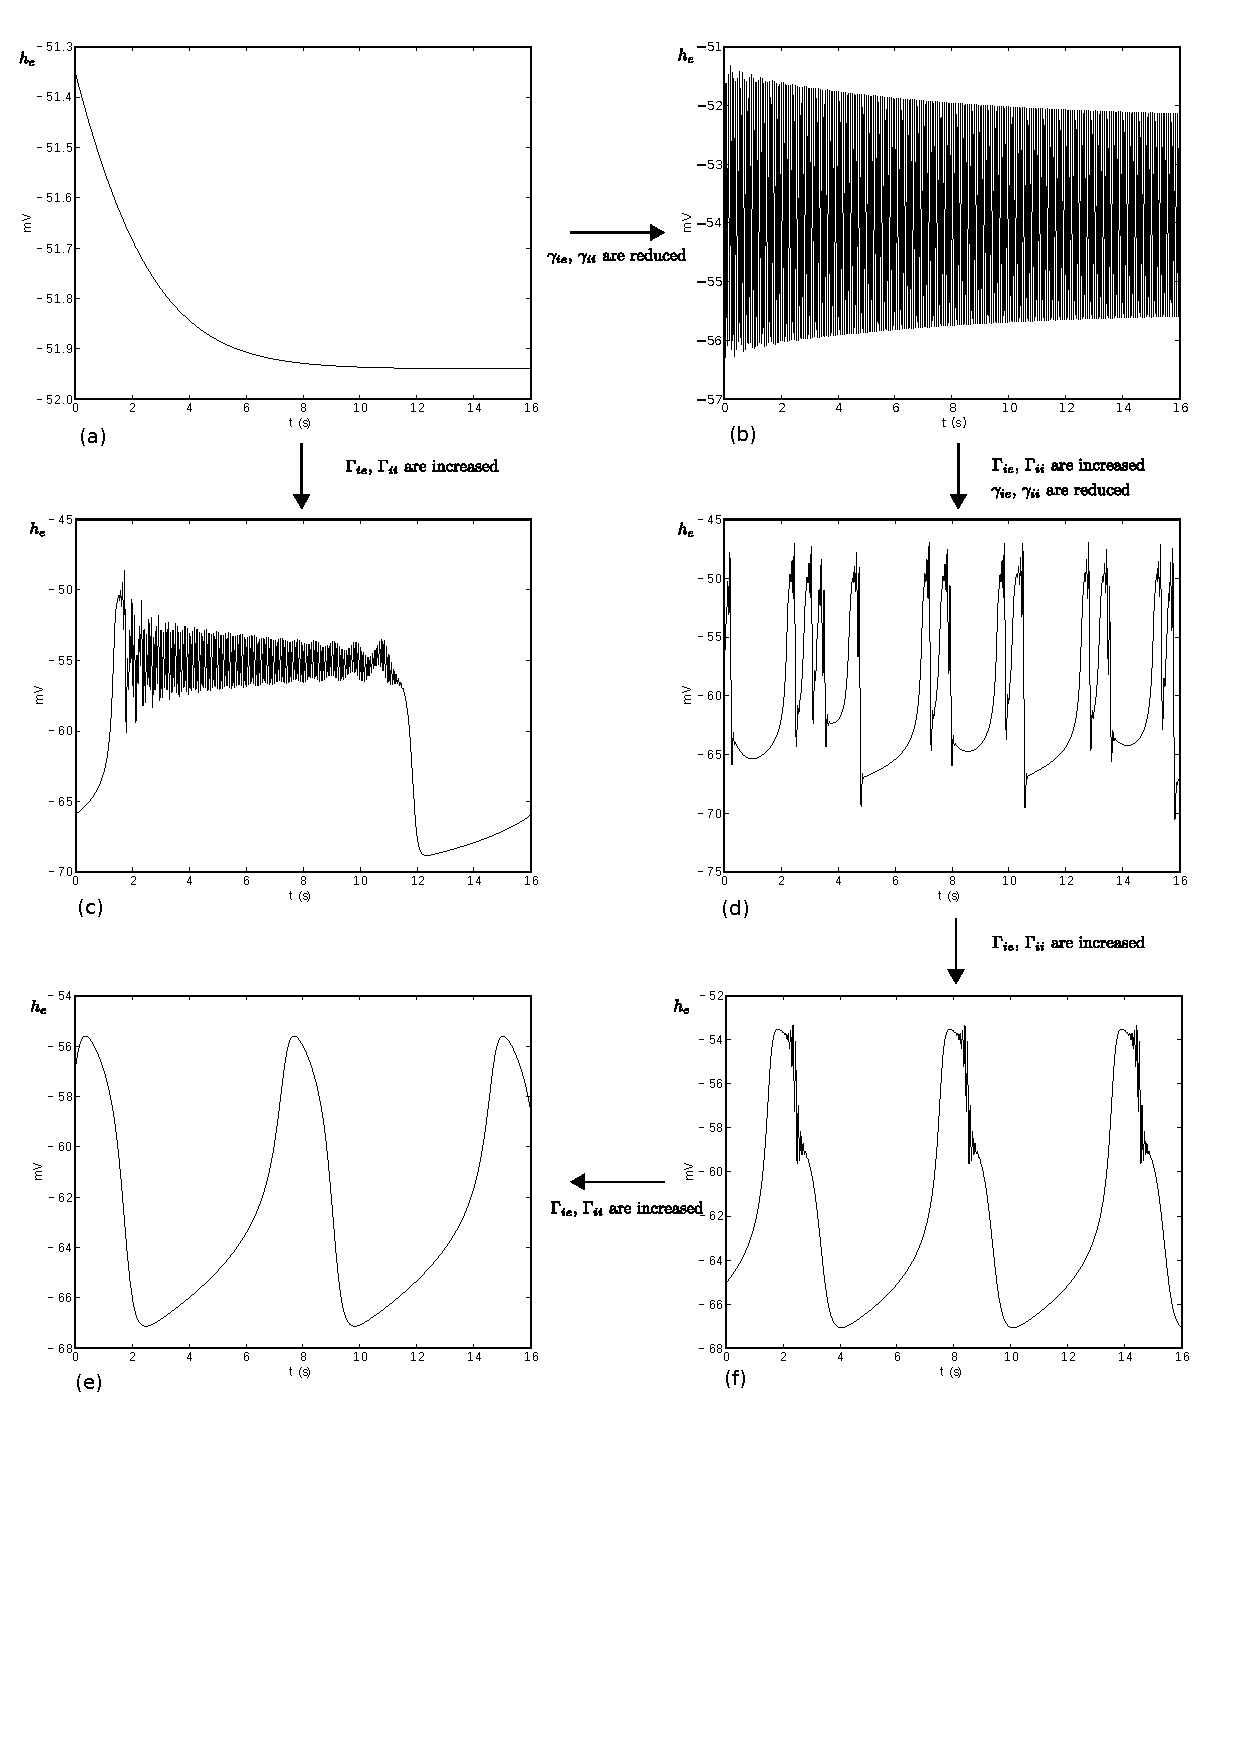
\includegraphics[scale=0.75]{frontiers-2012-working-images/figure-1-thal.pdf}
	\label{fig:00143}
	\caption{Mean excitatory soma membrane potential $h_e$ for a simulated induction of anaesthesia using the TA model. 
Reductions in inhibitory post synaptic potential rate constants ($\gamma_{ii}$ and $\gamma_{ie}$) and increases in inhibitory post synaptic potential peak amplitudes ($\Gamma_{ii}$ and $\Gamma_{ie}$) are performed to simulate known GABAergic anaesthetic action. Simulated induction brings about BS in (c), (d), (f) and slow waves in (e).
\\
(Please refer to the appendix for the parameters used in this simulation.)
}
\end{figure}

\begin{figure}
	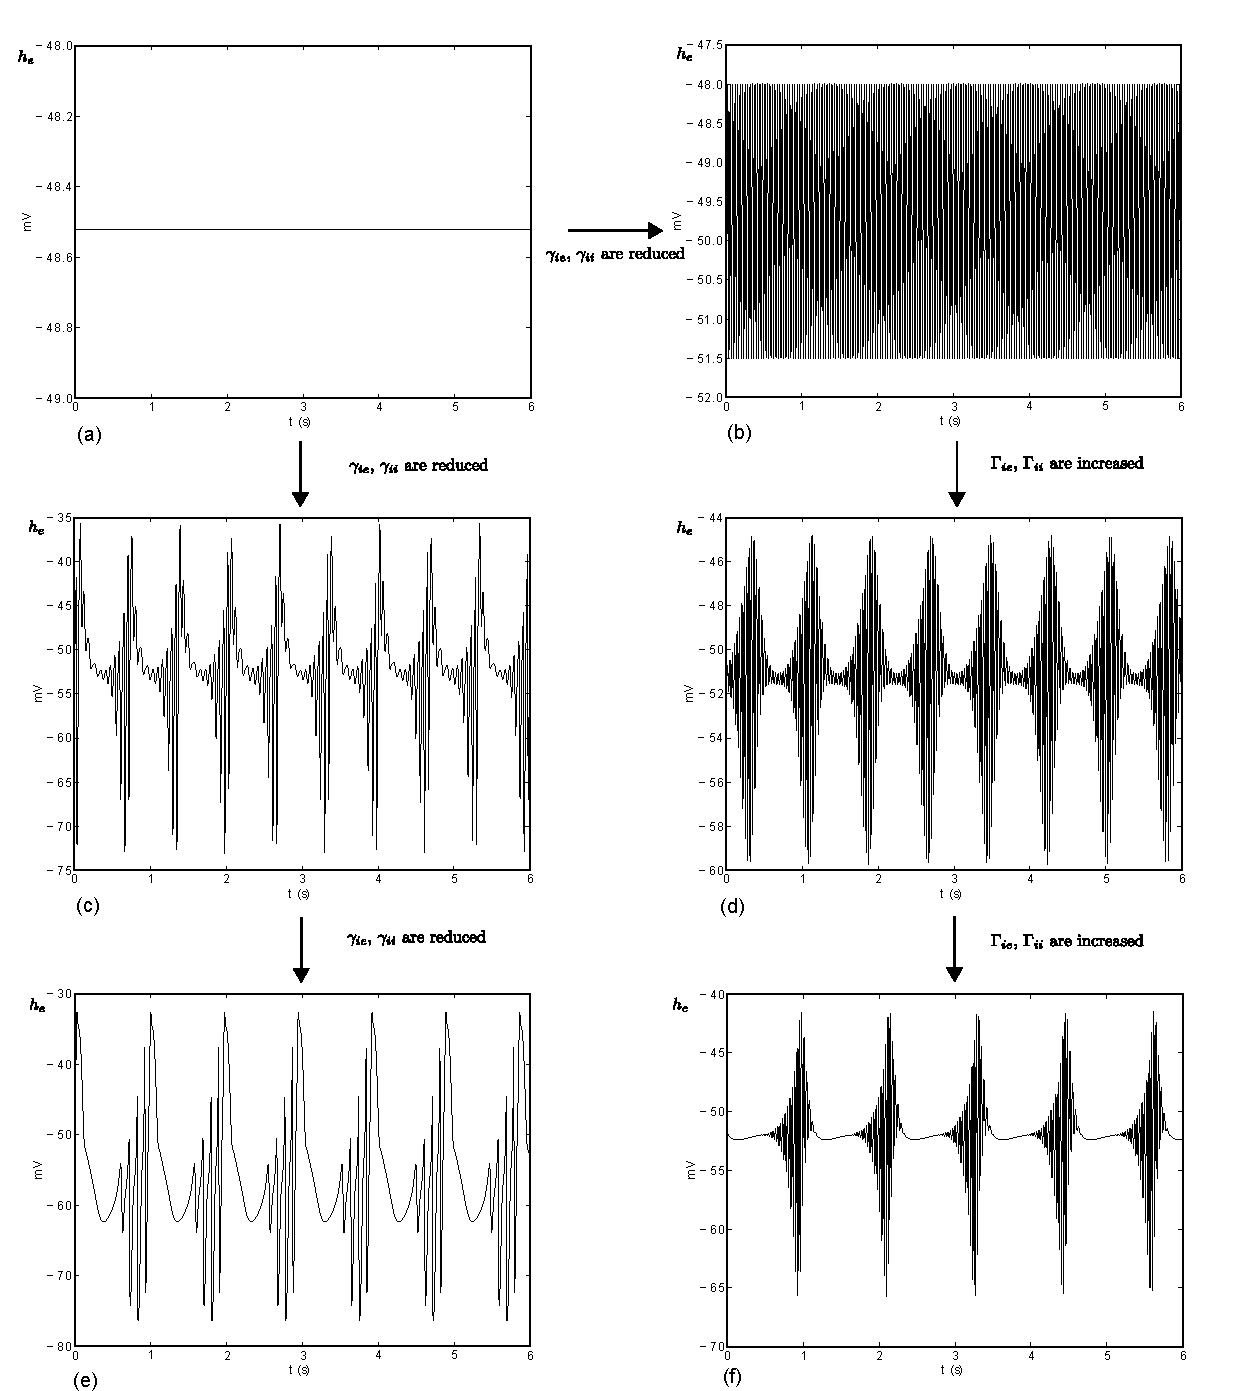
\includegraphics[scale=0.75]{frontiers-2012-working-images/figure-2-intra.pdf}
	\label{fig:intra_gamma}
	\caption{Mean excitatory soma membrane potential $h_e$ for a simulated induction of anaesthesia using the SIRU model. 
Reductions in inhibitory post synaptic potential rate constants ($\gamma_{ii}$ and $\gamma_{ie}$) and increases in inhibitory post synaptic potential peak amplitudes ($\Gamma_{ii}$ and $\Gamma_{ie}$) are performed to simulate known GABAergic anaesthetic action. Simulated induction of anaesthesia brings about BS in (c), (d), (e), (f). Simulated induction brings about variation in inter burst periods, as can be seen to occur between (c) and (e), (d) and (f).\\
(Please refer to the appendix for the parameters used in this simulation.)\\
}
\end{figure}

\begin{figure}
	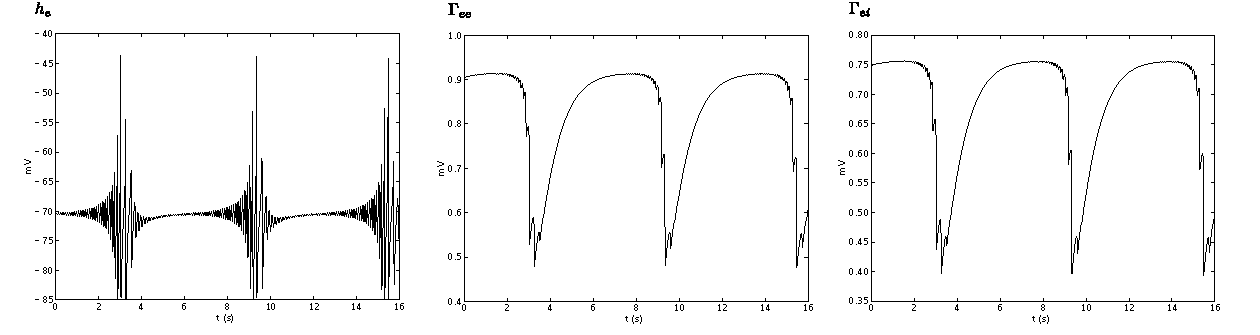
\includegraphics[scale=0.75]{frontiers-2012-working-images/figure-3-intra.pdf}
      \label{fig:emerging_slow_intra}
	\caption{The SIRU model represents intracellular and synaptic resource utilisation as a reduction in the excitatory peak PSPs ($\Gamma_{ee}$ and $\Gamma_{ei}$). The emergence of simulated BS within this model is accompanied by low frequency oscillations in the excitatory peak PSPs ($\Gamma_{ee}$ and $\Gamma_{ei}$). 
	(Please refer to the appendix for the parameters used in this simulation.)}
\end{figure}

\begin{figure}
	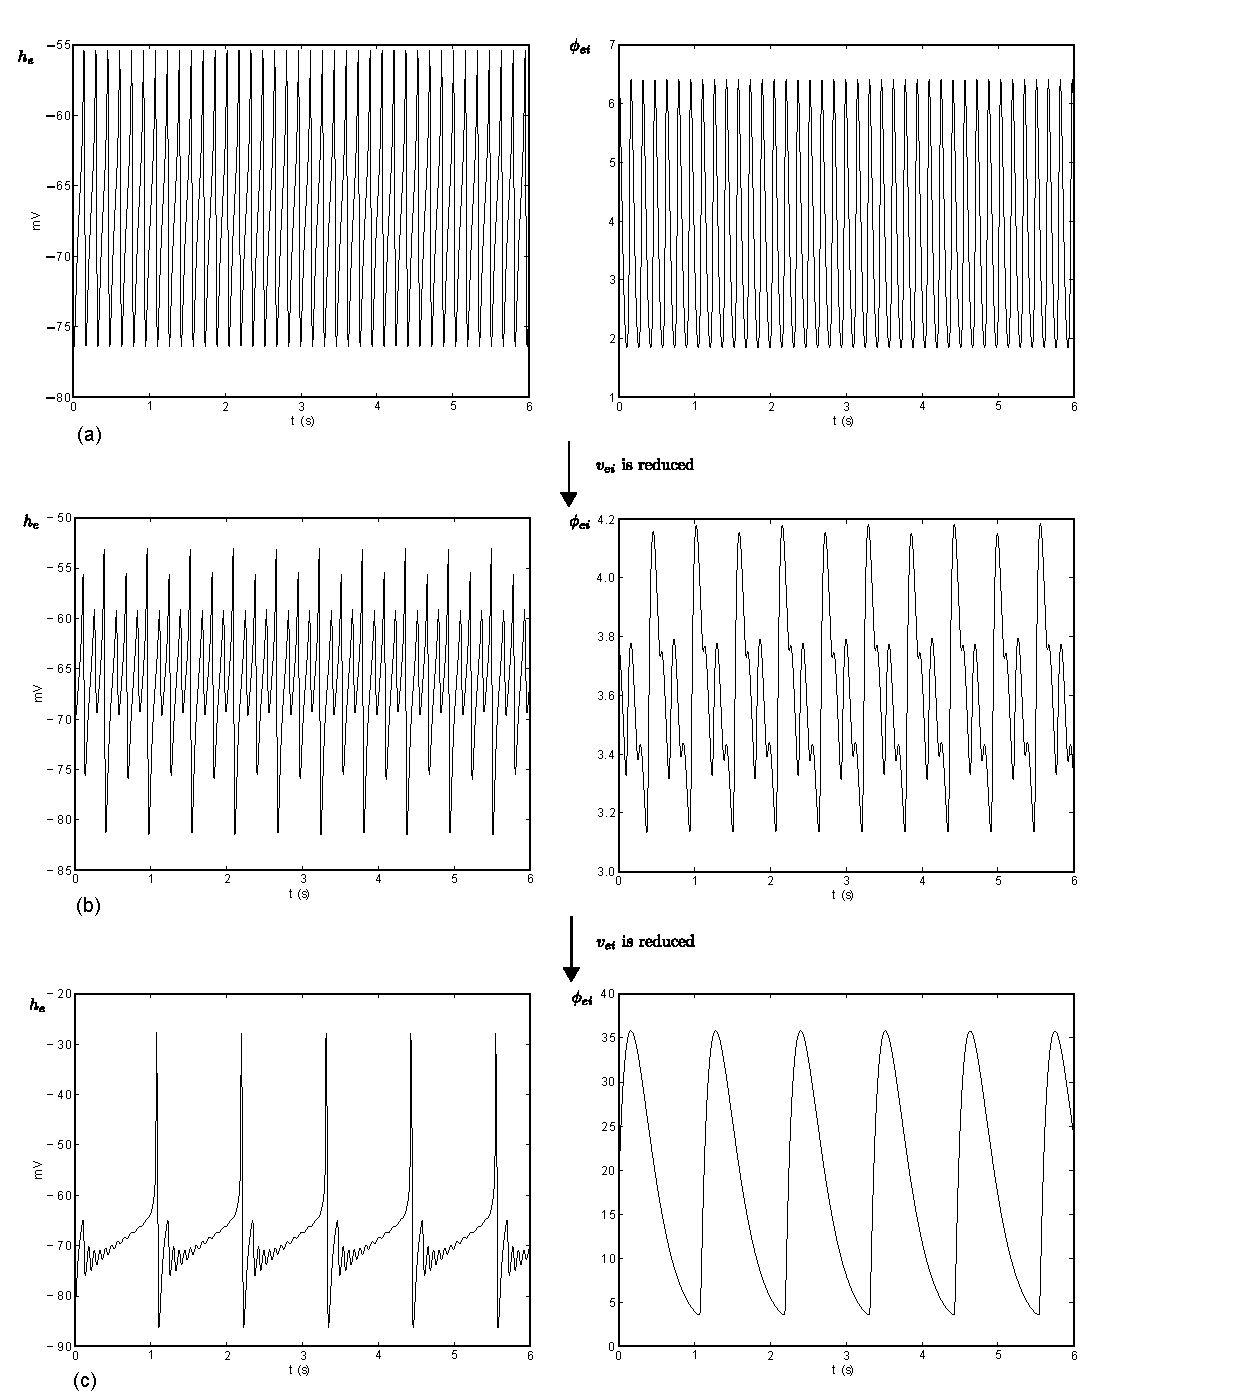
\includegraphics[scale=0.75]{frontiers-2012-working-images/figure-4-phi.pdf}
	\label{fig:phi_dyn}
	\caption{The reduction of conduction velocities ($v_{ee}$, $v_{ei}$) in the long range coupling system ($\phi_{ee}$, $\phi_{ei}$) brings low frequency oscillations that accompany simulated BS. \\
	(a) Sustained limit cycle behaviour with $\phi_{ei}$ operating on the same timescale as the coupled inhibitory/excitatory system ($h_e$).\\
           (b) $v_{ei}$ is reduced.\\
 (c) a further reduction of $v_{ei}$ from its value in (b) brings BS in conjunction with low frequency oscillations in the long range coupling system ($\phi_{ei}$).\\
(Please refer to the appendix for the parameters used in this simulation.)}
\end{figure}

\begin{figure}
	\begin{subfigure}[b]{0.5\textwidth}
		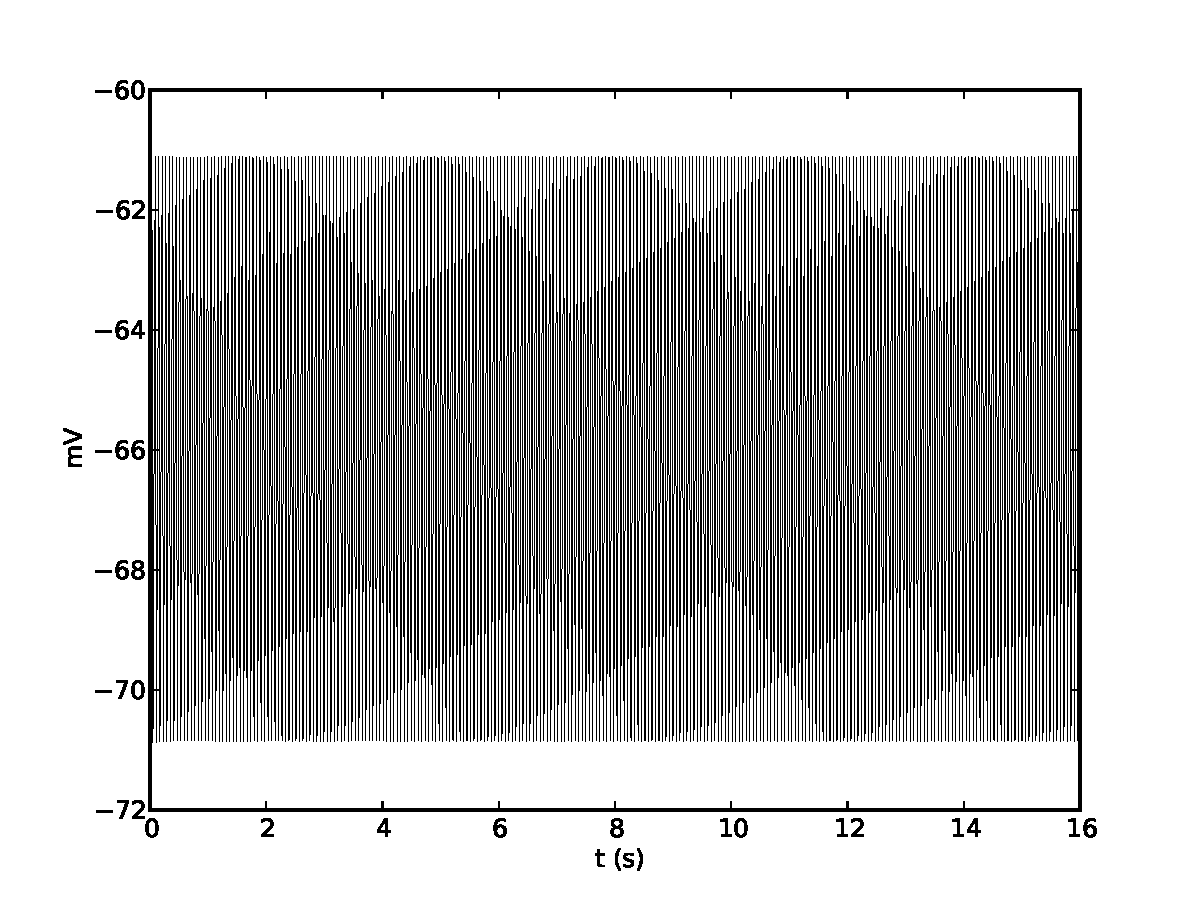
\includegraphics[scale=0.32]{frontiers-2012-images-revised/effect_gamma_ee_yml-00416_ode-phi-burst_yml-phi-mod-1_2-2-1-_yml-he-phi.pdf}
		\caption{$h_e$}
	\end{subfigure}
	\begin{subfigure}[b]{0.5\textwidth}
		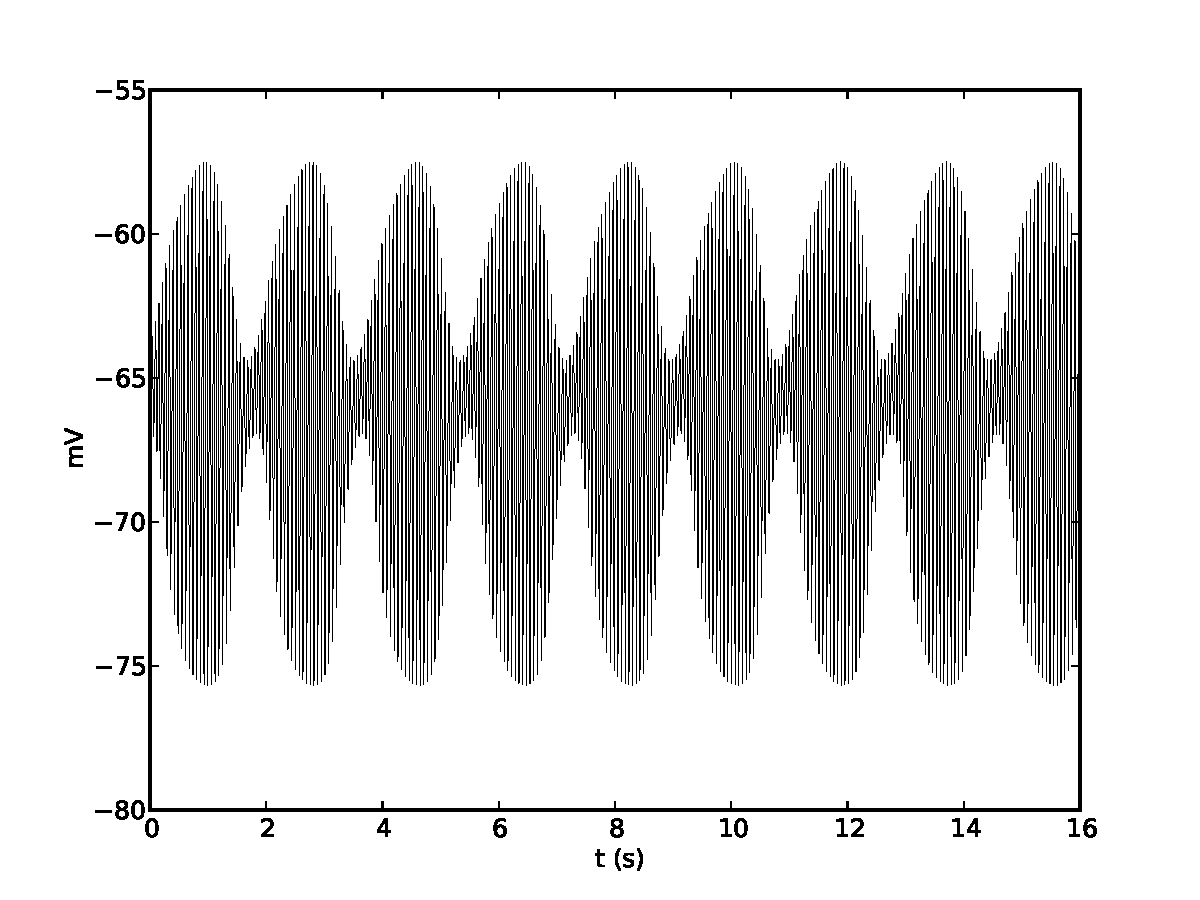
\includegraphics[scale=0.32]{frontiers-2012-images-revised/effect_gamma_ee_yml-00416_ode-phi-burst_yml-phi-mod-1_1-2-1-_yml-he-phi.pdf}
		\caption{$h_e$}
	\end{subfigure}
	\begin{subfigure}[b]{0.5\textwidth}
		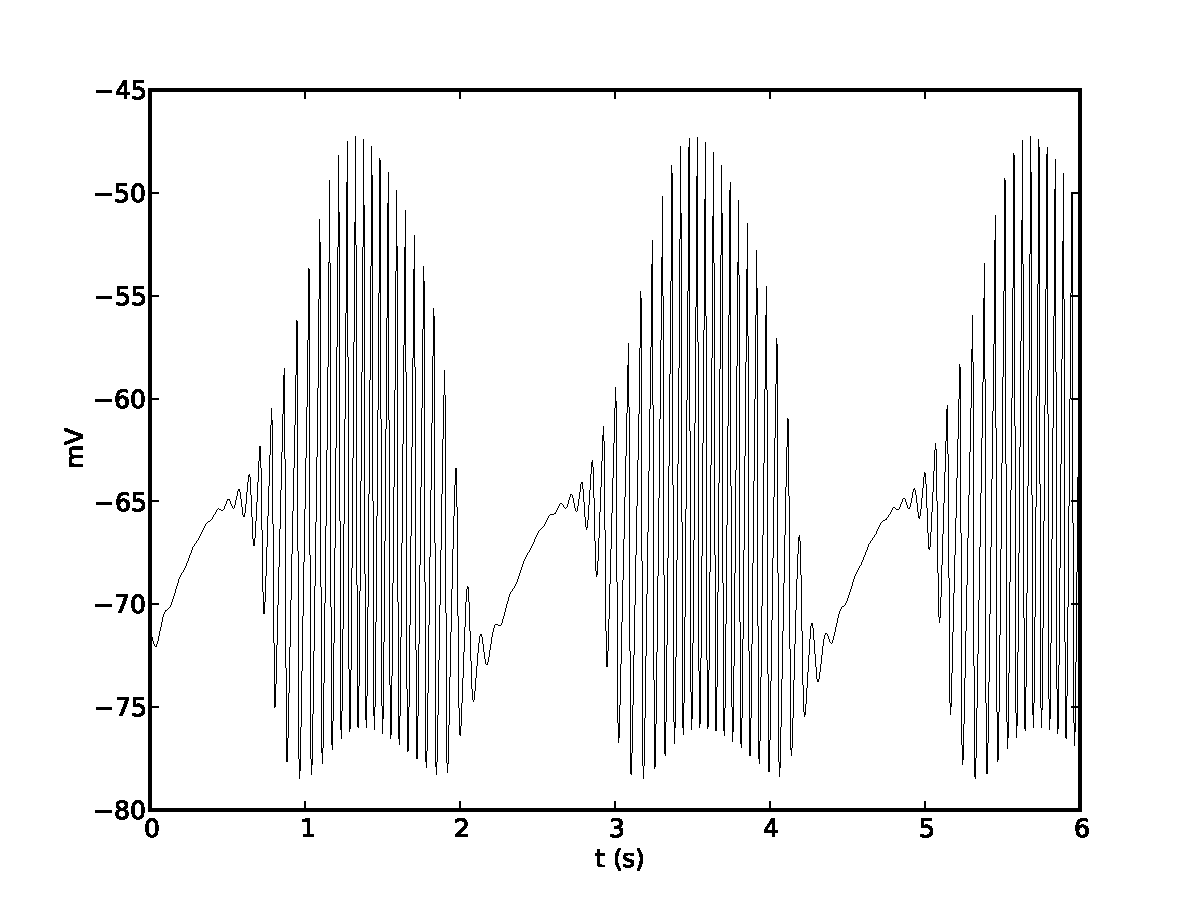
\includegraphics[scale=0.32]{frontiers-2012-images-revised/effect_gamma_ee_yml-00416_ode-phi-burst_yml-phi-mod-0_7-2-1-_yml-he-phi.pdf}
		\caption{$h_e$}
	\end{subfigure}

	\label{fig:phi_fast_var}
	\caption{Simulated induction of anaesthesia along with long range coupling $\phi_{ei}$ operating on a slowed timescale.\\
	(a) Sustained limit cycle behaviour.\\
           (b) Simulated anaesthetic induction was performed by a reduction in $\gamma_{ii}$ and $\gamma_{ie}$ bring about a modulation in spiking amplitude\\
           (b) A further reduction in $\gamma_{ii}$ and $\gamma_{ie}$ from their values in (b) brings about BS\\
	(Please refer to the appendix for the parameters used in this simulation.)}
\end{figure}


\section{Discussion}

\subsection{Long range coupling}
Although at this stage there is currently little evidence to suggest anaesthetics slow conduction velocities, it is
widely documented that axonal conduction velocities are significantly decreased in hypothermia. Decreases of up to 5\%
per $^{\circ}{\rm C}$ for conduction velocity have been reported (Waxman 1980) .

As BS has been observed associated with hypothermia(Schwartz et al, 1989; Akrawi et al 1996), we can conclude that  a slow system emerging in the long range coupling via a slowing of axonal conduction velocity is a possible route
to BS.

\subsection{Onset of BS may emerge partially or entirely from parametric changes in the coupled inhibitory/excitatory system}
Anaesthetic induction was simulated through the variation of model parameters ($\gamma_{ik}, \Gamma_{ik}$). All of these parameters are present in the cannonical model and are related to the coupled excitatory/inhibitory system. It was seen that variation of these parameters could instigate BS while leaving the slow timescale system parameters unchanged. These parametric changes were also observed to produce widely varying bursting dynamics. The transition from tonic spiking to bursting was not always observed to follow a parametric contour that was consistent with the induction of anaesthesia.

A parametric alteration in the long range coupling produced a slow timescale system that underlay the simulated BS. Along with this a variation of model parameters ($\gamma_{ik}, \Gamma_{ik}$) was able to instigate BS and vary its dynamics in the presence of this emergent slow timescale system.

There are still important questions outstanding regarding the effects of anaesthetics and their relationship to BS. Present knowledge of the effects of anaesthetics on parameters of the mean field model of Liley et al is restricted to cannonical model parameters. The effects of anaesthesia on the introduced slow systems in this investigation is not yet understood. 

It is clear from this investigation that the changes in parameters that relate to known effects of anaesthetics can affect and induce BS and these changes may present themselves as a fundamental mechanism in the onset of BS. A larger scale analysis of parametric variation is needed to help determine the underlying trigger and topological structure relating to BS.

\subsection{Multiple origins for bursting possible}
This investigation has presented three possible mechanisms in which a slow timescale system underlying BS could emerge. Intra-cortical (long range coupling and SIRU) and extra-cortical (TA) mechanisms were presented and all were able to display simulated BS. All of these mechanisms are physiologically plausible and it is thus conceivable that multiple modes of BS arising from anaesthesia are possible. Interactions between muliple slow timescale systems may also be involved. As each slow timescale system presented in this investigation was considered in isolation further work is needed to investigate the interactions between the introduced and emergent slow timescale systems.

\subsection{Further investigations}
The current investigations have focussed on the spatially homogeneous case for the model of Liley et al. (i.e. $\nabla^2 =
0$ in \ref{eq:phi}). The cortical phase synchrony(ref?) of burst suppression therefore has not as yet been investigated.

This investigation considered each emergent slow timescale system in isolation. There has not as yet been an investigation of the
interactions between the presented emergent slow timescale system in a unified model covering all the presented augmentations in this investigation.

A greater understanding of the effect that variation of the cannonical model parameters known to vary under anaesthesia have on instigating BS is needed. This is essential to help pinpoint the conditions under which anaesthesia triggers BS.

\appendix
\section{Appendix}
\subsection{Simulation Parameter Sets}
\subsubsection{Parameters for simulation presented in figure \ref{fig:00143}}
\paragraph{Common parameters}
$\Lambda_{ee} = 0.97961, \Lambda_{ei} = 0.97961, N^{\alpha}_{ee} = 3218.25773, N^{\alpha}_{ei} = 1725.76994,
N^{\beta}_{ee} = 2555.55532, N^{\beta}_{ei} = 3955.40197, N^{\beta}_{ie} = 558.83565, N^{\beta}_{ii} = 805.76418,
\Gamma_{ee} = 0.15173, \Gamma_{ei} = 0.27124, 
 g = 0.7, \gamma_{ee} = 0.31475, \gamma_{ei} = 0.24595,  h_e^{rest} = -66.96585, h_{ee}^{eq} = 0.03533, h_{ei}^{eq} = -6.84352,
h_i^{rest} = -77.90611, h_{ie}^{eq} = -85.52639, h_{ii}^{eq} = -85.43499,
\mu_e = -50.73253, \mu_i = -51.66220,  \hat{p}_{ee} = 2.16873, \hat{p}_{ei} = 2.43422, p_{ie} = 0.0, p_{ii} = 0.0, \phi_{ie} = 0,
\phi_{ii} = 0, S_e^{max} = 0.101903, S_i^{max} = 0.469, \sigma_e = 6.02439, \sigma_i = 4.21866,
\rho_e = 800.0, \rho_i = 3200.0, \tau_e = 139.779, \tau_i = 22.5263, \tau^{slow} = 6988.95,
v_{ee} = 0.68140, v_{ei} = 0.68140$
\paragraph{Modified simulation parameters}
(a) $\gamma_{ie} = 0.07924$, $\gamma_{ii} = 0.06251$, $\Gamma_{ie} = 0.69872$, $\Gamma_{ii} = 0.69021$\\
(b) $\gamma_{ie} = 0.05209$, $\gamma_{ii} = 0.06604$, $\Gamma_{ie} = 0.69872$, $\Gamma_{ii} = 0.69021$\\
(c) $\gamma_{ie} = 0.05209$, $\gamma_{ii} = 0.06604$, $\Gamma_{ie} = 0.97821$, $\Gamma_{ii} = 0.96629$\\
(d) $\gamma_{ie} = 0.05943$, $\gamma_{ii} = 0.04688$, $\Gamma_{ie} = 0.69872$, $\Gamma_{ii} = 0.69021$\\
(e) $\gamma_{ie} = 0.05209$, $\gamma_{ii} = 0.06604$, $\Gamma_{ie} = 1.81668$, $\Gamma_{ii} = 1.79454$\\
(f) $\gamma_{ie} = 0.05209$, $\gamma_{ii} = 0.06604$, $\Gamma_{ie} = 1.53719$, $\Gamma_{ii} = 1.51845$\\



\subsubsection{Parameters for simulation presented in figure \ref{fig:intra_gamma}}
\paragraph{Common parameters}
$\Lambda_{ee} = 0.77255, \Lambda_{ei} = 0.77255, N^{\alpha}_{ee} = 4111.52244, N^{\alpha}_{ei} = 2939.96568,
N^{\beta}_{ee} = 2121.71866, N^{\beta}_{ei} = 3394.56035, N^{\beta}_{ie} =  846.44498, N^{\beta}_{ii} = 178.04925,
\hat{\Gamma}_{ee} =  0.10367, \hat{\Gamma}_{ei} = 1.21771, 
\chi_{ee} = 420.196, \chi_{ei} = 420.196, \gamma_{ee} = 0.07383,
\gamma_{ei} = 0.82956, h_e^{rest} = -68.11516,
h_{ee}^{eq} = -6.87622, h_{ei}^{eq} = -10.85385, h_i^{rest} = -79.2805, h_{ie}^{eq} = -78.14073,
h_{ii}^{eq} = -89.33821, \mu_e = -45.58067, \mu_i = -46.22321,
p_{ee} = 3.12714, p_{ei} = 5.15692,
p_{ie} = 0.0, p_{ii}: 0.0, \phi_{ie} = 0, \phi_{ii} = 0, S_e^{max} = 0.11240, S_i^{max} = 0.17063,
\sigma_e = 3.61819399, \sigma_i = 3.12887627, \tau_e = 21.0098, \tau_i = 77.73, 
\tau^{slow}_{ee} = 420.196, \tau^{slow}_{ei} = 420.196, v_{ee} = 0.96791, v_{ei} = 0.96791$
\paragraph{Modified simulation parameters}
(a) $\gamma_{ie} = 1.80757$, $\gamma_{ii} = 0.42574$, $\Gamma_{ie} = 1.36689$, $\Gamma_{ii} = 0.99961$\\
(b) $\gamma_{ie} = 1.08454$, $\gamma_{ii} = 0.25544$, $\Gamma_{ie} = 1.36689$, $\Gamma_{ii} = 0.99961$\\
(c) $\gamma_{ie} = 0.32536$, $\gamma_{ii} = 0.07663$, $\Gamma_{ie} = 1.36689$, $\Gamma_{ii} = 0.99961$\\
(d) $\gamma_{ie} = 1.08454$, $\gamma_{ii} = 0.25544$, $\Gamma_{ie} = 2.73378$, $\Gamma_{ii} = 1.99922$\\
(e) $\gamma_{ie} = 0.18076$, $\gamma_{ii} = 0.04257$, $\Gamma_{ie} = 1.36689$, $\Gamma_{ii} = 0.99961$\\
(f) $\gamma_{ie} = 1.08454$, $\gamma_{ii} = 0.25544$, $\Gamma_{ie} = 4.10068$, $\Gamma_{ii} = 2.99883$\\

\subsubsection{Parameters used for figure \ref{fig:emerging_slow_intra}}
$\Lambda_{ee} = 0.41833, \Lambda_{ei} =  0.41833, N^{\alpha}_{ee} = 3524.12798, N^{\alpha}_{ei} = 1178.47583,
N^{\beta}_{ee} = 4567.01614, N^{\beta}_{ei} = 2946.02934, N^{\beta}_{ie} = 705.66451, N^{\beta}_{ii} = 155.69243,
\hat{\Gamma}_{ee} = 1.03021, \hat{\Gamma}_{ei} = 1.24548, \Gamma_{ie} = 3.32228, \Gamma_{ii} = 2.28976,
\chi_{ee} = 1290.08, \chi_{ei} = 1290.08, \gamma_{ee} = 0.71337, \gamma_{ei} = 0.53411,
\gamma_{ie} = 0.35526, \gamma_{ii} = 0.02911, h_e^{rest} = -79.27218, h_{ee}^{eq} = -19.32193,
h_{ei}^{eq} = -8.30757, h_i^{rest} = -76.08372, h_{ie}^{eq} = -85.45751, h_{ii}^{eq} = -84.48223,
\mu_e: -54.37736, \mu_i: -54.60727, p_{ee}: 6.83303, p_{ei}: 9.26794, p_{ie}: 0.0, p_{ii}: 0.0,
\phi_{ie}: 0, phi_{ii}: 0, S_e^{max} = 0.0637, S_i^{max} = 0.08382, \sigma_e = 4.16944,
\sigma_i = 2.1261, \tau_e = 73.3, \tau_i = 75.2, \tau^{slow}_{ee} = 1612.6,
  \tau^{slow}_{ei}: 1612.6, v_{ee} = 0.83906, v_{ei} = 0.83906$

\subsubsection{Parameters for simulation presented in figure \ref{fig:phi_dyn}}
\paragraph{Common parameters}
$\Lambda_{ee} = 1.94376, \Lambda_{ei} = 0.19438, N^{\alpha}_{ee} = 2661.2743, N^{\alpha}_{ei} = 2415.41369,
N^{\beta}_{ee} = 4537.65784, N^{\beta}_{ei} = 4285.31857, N^{\beta}_{ie} = 496.40152, N^{\beta}_{ii} = 989.81774,
\Gamma_{ee} = 0.42627, \Gamma_{ei} = 1.71876, \Gamma_{ie} = 0.85708, \Gamma_{ii} = 1.32239,
\gamma_{ee} = 0.78950, \gamma_{ei} = 0.82632, \gamma_{ie} = 0.14777,
\gamma_{ii} = 0.04887, h_e^{rest} = -75.54581, h_{ee}^{eq} = -16.50733, h_{ei}^{eq} = -2.72987,
h_i^{rest} = -75.55675, h_{ie}^{eq} = -88.67197, h_{ii}^{eq} = -85.43396, \mu_e = -42.50181, \mu_i = -48.70101, 
p_{ee} = 7.18587, p_{ei} = 6.79444, p_{ie} = 0.0, p_{ii} = 0.0, phi_{ie} = 0,
\phi_{ii} = 0, S_e^{max} = 0.45018, S_i^{max} = 0.07468, \sigma_e = 5.02482,
\sigma_i = 3.22531, \tau_e = 38.9, \tau_i = 137.859, v_{ee} = 0.82458$
\paragraph{Modified simulation parameters}
(a) $v_{ei} = 0.16492$\\
(b) $v_{ei} = 0.04123$\\
(c) $v_{ei} = 0.02474$\\


\subsubsection{Parameters for simulation presented in figure \ref{fig:phi_fast_var}}
\paragraph{Common parameters}
$\Lambda_{ee} = 0.33012064, \Lambda_{ee} = 0.033012064, N^{\alpha}_{ee} =  2342.99410942, N^{\alpha}_{ei} =  2635.01259668,
N^{\beta}_{ee} =  4016.1981429, N^{\beta}_{ei} =  4356.20256437, N^{\beta}_{ie} =  634.73935613, N^{\beta}_{ii} =  473.38388612,
\Gamma_{ee} = 0.13699266, \Gamma_{ei} = 0.4439827, \Gamma_{ie} = 2.85705762, \Gamma_{ii} = 0.28147566, \gamma_{ee} = 0.244953287255, \gamma_{ei} = 0.82969594, h_e^{rest} = -61.7485641, h_{ee}^{eq} = 5.73011624, h_{ei}^{eq} = 2.099135,
h_i^{rest} = -64.46142322, h_{ie}^{eq} = -81.67044311, h_{ii}^{eq} = -82.29433835, \mu_e = -53.10048735, \mu_i = -53.68380602, p_{ee} = 3.6997382629, p_{ei} = 0.60015865013, p_{ie} = 0.0, p_{ii} = 0.0, \phi_{ie} = 0,
\phi_{ii} = 0, S_e^{max} = 0.0930382, S_i^{max}= 0.0648537, \sigma_e = 4.64535035,
\sigma_i = 3.10925431, \tau_e = 86.1876, \tau_i = 65.0391, \tau^{slow} = 1, v_{ee} = 0.160606,
  v_{ei} = 0.160606$

\paragraph{Modified simulation parameters}
(a) $\gamma_{ii} = 0.10813$ and $\gamma_{ie} = 0.54945$\\
(b) $\gamma_{ii} = 0.09913$ and $\gamma_{ie} = 0.50367$\\
(c) $\gamma_{ii} = 0.06308$ and $\gamma_{ie} = 0.32052$\\

\bibliography{frontiers_in_neuroscience_oct_2012}


\end{document}

